\section{Background}

% \subsection{Introduction and Recent Developments}

% \begin{frame}
% \frametitle{Recent Developments in Neutral Atom Quantum Computing}

% % \begin{itemize}
% %     \item \textbf{Microsoft and Atom Computing Collaboration} \\
% %     \href{https://www.microsoft.com/en-us/research/blog/microsoft-and-atom-computing-collaborate-on-quantum-supercomputer}{\footnotesize{microsoft.com/en-us/research/blog/microsoft-and-atom-computing-collaborate-on-quantum-supercomputer}}
    
% %     \item \textbf{Modular Quantum System-on-Chip Development} \\
% %     \href{https://www.nature.com/articles/s41586-024-07371-7}{\footnotesize{nature.com/articles/s41586-024-07371-7}}
    
% %     \item \textbf{Fault-Tolerant Quantum Computation with High-Rate qLDPC Codes} \\
% %     \href{https://arxiv.org/abs/2408.12345}{\footnotesize{arxiv.org/abs/2408.12345}}
% % \end{itemize}
% % \end{frame}

\subsection{Neutral Atom Quantum Computing Hardware}
\begin{frame}{Comparison of Quantum Computing Platforms}

\small % Reduce font size for the table
\begin{table}[h!]
\centering
\begin{tabular}{lccc}
\toprule
 & \textbf{Superconducting} & \textbf{Trapped-Ion} & \textbf{Neutral Atom} \\
\midrule
\textbf{Implementation} & Josephson Junctions & Trapped Ions & Optical Lattices \\
\textbf{Gate Speed} & $\sim$ ns & $\sim$ ms & $\sim$ $\mu$s \\
\textbf{Coherence Time} & $\sim$$\mu$s & $\sim$10 s & $\sim$1 s \\
\textbf{Fidelity} & 99.9\% & 99.99\% & 99\% \\
\textbf{Scalability} & Medium & Limited & High Potential \\
\bottomrule
\end{tabular}
\end{table}

\end{frame}

\begin{frame}{Overview of Neutral Atom Quantum Computing}
    \begin{itemize}
        \item \textbf{Qubits:} Individual neutral atoms (e.g., rubidium, cesium)
        \item \textbf{Trapping Methods:} Optical tweezers, optical lattices
        \item \textbf{Encoding:} Internal atomic states (hyperfine ground states)
        \item \textbf{Interactions:} Mediated via Rydberg state excitation
    \end{itemize}
\end{frame}

\begin{frame}{Common Atoms Used in Neutral Atom Devices}
  \begin{itemize}
    \item \textbf{Alkali Atoms:} Rubidium (Rb), Cesium (Cs)
    \item \textbf{Alkaline-Earth-Like Atoms:} Strontium (Sr), Ytterbium (Yb)
  \end{itemize}
  \centering
  \includegraphics[width=0.7\textwidth]{images/Colour_18-col_PT_with_labels.png}
\end{frame}

\begin{frame}{Hardware Workflow}
    \begin{columns}
        \begin{column}{.3\textwidth}
            \begin{enumerate}
                \item Metal Vapor Source
                \item Atomic Beam Formation
                \item Laser Cooling Techniques
                \item Optical Trapping (Lattice)
                \item Atom Rearrangement
            \end{enumerate}
        \end{column}
        \begin{column}{.7\textwidth}
            \begin{figure}
                \includegraphics[width=.9\textwidth]{images/image.png}
                \caption{Overview of the Main Hardware Components in a Quantum Processor}
            \end{figure}
        \end{column}
    \end{columns}
\end{frame}

\begin{frame}{Optical Traps and Tweezers}
  \begin{itemize}
    \item \textbf{Atom Trapping Methods:}
      \begin{itemize}
        \item Optical dipole traps
        \item Optical tweezers created by focused laser beams
      \end{itemize}
    \item \textbf{Array Configurations:}
      \begin{itemize}
        \item One-, two-, or three-dimensional setups
      \end{itemize}
    \item \textbf{Dynamic Control:}
      \begin{itemize}
        \item Reloading and rearrangement of atoms
        \item Enhances scalability and qubit manipulation
      \end{itemize}
  \end{itemize}
\end{frame}

\subsection{Quantum Gates and Operations}

\begin{frame}{Single-Qubit Gates}
  \begin{itemize}
    \item \textbf{Quantum State Manipulation:}
      \begin{itemize}
        \item Laser pulses induce Rabi oscillations between qubit states \( |0\rangle \) and \( |1\rangle \)
        \item Control via Rabi frequency (\( \Omega(t) \)) and detuning (\( \Delta(t) \))
      \end{itemize}
    \item \textbf{Hamiltonian:}
      \[
          \frac{H_1(t)}{\hbar} = \frac{\Omega(t)}{2} |0\rangle\langle 1| + \frac{\Omega^*(t)}{2} |1\rangle\langle 0| - \Delta(t) |1\rangle\langle 1|
      \]
    \item \textbf{Implementation Techniques:}
      \begin{itemize}
        \item Single- or two-photon transitions
        \item Individual or global laser addressing
      \end{itemize}
  \end{itemize}
\end{frame}

\begin{frame}{Two-Qubit Gates via Rydberg Blockade}
    \begin{itemize}
        \item \textbf{Rydberg Blockade Mechanism:}
        \begin{itemize}
            \item Prevents simultaneous excitation of adjacent atoms to Rydberg states
            \item Interaction strength characterized by the blockade radius \( r_b \)
        \end{itemize}
        \item \textbf{Blockade Radius:}
        \[
            r_b \simeq \left( \frac{C_6}{\hbar \Omega_r} \right)^{1/6}
        \]
        \item \textbf{Enhanced Connectivity:}
        \begin{itemize}
            \item Enables entanglement between non-neighboring qubits
            \item Facilitates complex quantum operations
        \end{itemize}
    \end{itemize}
\end{frame}
\begin{frame}{blockade radius}
    In Rydberg state, atoms exhibit strong long-range interactions, leading to a blockade effect where the excitation of one atom can prevent the excitation of nearby atoms.

    
    \centering
    \scalebox{0.8}{% \documentclass{standalone}
% \usepackage{tikz}
% \usetikzlibrary{calc}
% \begin{document}

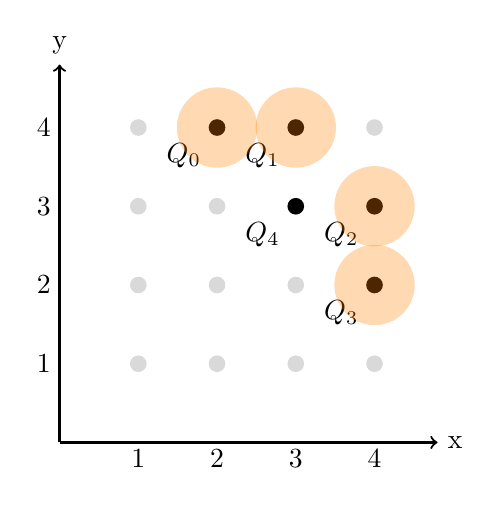
\begin{tikzpicture}
    % Helper styles for better readability
    \tikzstyle{unoccupied}=[fill=gray!30, circle, minimum size=6pt, inner sep=0pt]
    \tikzstyle{occupied}=[fill=black, circle, minimum size=6pt, inner sep=0pt]
    \tikzstyle{rydbery_circle}=[fill=orange, opacity=0.3]

    \begin{scope}[shift={(0,0)}]
        % Axes
        \draw[->, thick] (0, 0) -- (4.8, 0) node[right] {x};
        \draw[->, thick] (0, 0) -- (0, 4.8) node[above] {y};

        % x and y labels
        \foreach \x in {1, 2, 3, 4} {
            \node at (\x, -0.2) {\x};
        }
        \foreach \y in {1, 2, 3, 4} {
            \node at (-0.2, \y) {\y};
        }
    
        % Unoccupied nodes - dashed circles
        \foreach \x in {1, 2, 3, 4} {
            \foreach \y in {1, 2, 3, 4} {
                \node[unoccupied] at (\x, \y) {};
            }
        }
        
        % SLM occupied nodes (filled circles)
        \foreach [count=\i from 0] \x/\y in {2/4, 3/4, 4/3, 4/2, 3/3} {
            \node[occupied, label=below left:{$Q_{\i}$}] at (\x, \y) {};
        }
        
        % rydbery laser(circled filled circles), r = 1
        \foreach \x/\y in {2/4, 3/4, 4/3, 4/2} {
            \fill[rydbery_circle] (\x, \y) circle (0.51);
        }
        % r=2
        % \foreach \x/\y in {2/4, 3/4, 4/3, 4/2} {
        %     \fill[rydbery_circle] (\x, \y) circle (1);
        % }
        
        % Title
        % \node[below] at ($(2.5,-0.5)$) {b)};
    \end{scope}

\end{tikzpicture}

% \end{document}
}
    \scalebox{0.8}{\input{images/gate_conf}}
\end{frame}
\begin{frame}{Multi-Qubit Gates}
    \begin{figure}
        \centering
        \includegraphics[width=0.8\linewidth]{images/multi-gate.png}
        \caption{Implementation of Multi-Qubit Gates Using Rydberg Interactions}
    \end{figure}
\end{frame}

% \subsection{Atom Shuttling and Connectivity Enhancement}

\begin{frame}{Atom Shuttling Techniques}
    \begin{itemize}
        \item \textbf{Dynamic Qubit Movement:}
        \begin{itemize}
            \item Transfer atoms between static (SLM-based) and dynamic (AOD-based) optical traps
            \item Maintains quantum coherence during movement
        \end{itemize}
        \item \textbf{Connectivity Benefits:}
        \begin{itemize}
            \item Enhances qubit interaction range without additional gates
            \item Reduces the need for SWAP operations, improving efficiency
        \end{itemize}
        \item \textbf{Dynamically Field-Programmable Qubit Arrays (FPQA):}
        \begin{itemize}
            \item Architecture focused on shuttling for flexible qubit arrangement
            \item Incorporates dedicated zones for entangling, measurement, and storage
        \end{itemize}
    \end{itemize}
\end{frame}

\begin{frame}{Visualization of Shuttling Process}
    \begin{columns}
        \begin{column}{.48\textwidth}
            \begin{figure}
                \includegraphics[width=.8\textwidth]{images/rearrange.png}
                \caption{Atom Movement Between Trap Sites}
            \end{figure}
        \end{column}
        \begin{column}{.48\textwidth}
            \begin{figure}
                \includegraphics[width=.8\textwidth]{images/dpqa.png}
                \caption{Dynamically Field-Programmable Qubit Array}
            \end{figure}
        \end{column}
    \end{columns}
\end{frame}

\subsection{Scalability and Noise Considerations}

\begin{frame}{Scalability Potential}
  \begin{itemize}
    \item \textbf{Customizable Geometries:}
      \begin{itemize}
        \item Atoms can be arranged in tailored configurations
      \end{itemize}
    \item \textbf{Long-Range Entanglement:}
      \begin{itemize}
        \item Rydberg interactions enable entanglement over larger distances
      \end{itemize}
    \item \textbf{Enhanced Connectivity via Shuttling:}
      \begin{itemize}
        \item Physical movement of qubits increases interaction possibilities
      \end{itemize}
  \end{itemize}
\end{frame}

\begin{frame}{Challenges in Scaling Up}
  \begin{itemize}
    \item \textbf{Cross-Talk Between Qubits:}
      \begin{itemize}
        \item Imperfect laser focus can cause unwanted interactions
        \item Mitigation requires precise control over laser parameters
      \end{itemize}
    \item \textbf{Maintaining Coherence:}
      \begin{itemize}
        \item Larger systems may experience reduced coherence times
        \item Requires improved isolation from environmental disturbances
      \end{itemize}
    \item \textbf{Reliable Atom Control:}
      \begin{itemize}
        \item Atom loss and decoherence during operations
        \item Necessitates advanced trapping and cooling techniques
      \end{itemize}
  \end{itemize}
\end{frame}
\begin{frame}{Comparison with Other Quantum Platforms}
    \begin{block}{Superconducting Qubits}
        \begin{itemize}
            \item Sensitive to electromagnetic noise and material defects
            \item Decoherence from charge and flux fluctuations
        \end{itemize}
    \end{block}
    \begin{block}{Trapped Ion Qubits}
        \begin{itemize}
            \item Susceptible to electric field variations
            \item Issues with motional heating and laser phase noise
        \end{itemize}
    \end{block}
    % \begin{block}{Photonic Qubits}
    %     \begin{itemize}
    %         \item Affected by photon loss and detector inefficiencies
    %         \item Less sensitive to thermal and environmental noise
    %     \end{itemize}
    % \end{block}
\end{frame}
% \subsection{Noise Sources and Mitigation Strategies}

% \begin{frame}{Noise Sources in Neutral Atom Quantum Computing}
%     \begin{itemize}
%         \item \textbf{Laser Noise:}
%         \begin{itemize}
%             \item Intensity fluctuations
%             \item Frequency and phase instability
%         \end{itemize}
%         \item \textbf{Atom Loss:}
%         \begin{itemize}
%             \item Collisions with residual gas particles
%             \item Photon scattering-induced heating
%         \end{itemize}
%         \item \textbf{Decoherence Mechanisms:}
%         \begin{itemize}
%             \item Spontaneous emission
%             \item Interaction with blackbody radiation
%         \end{itemize}
%         \item \textbf{Motional Decoherence:}
%         \begin{itemize}
%             \item Residual thermal motion of atoms
%             \item Fluctuations in trapping potentials
%         \end{itemize}
%         \item \textbf{Control Field Errors:}
%         \begin{itemize}
%             \item Beam imperfections
%             \item Timing jitter in control pulses
%         \end{itemize}
%         \item \textbf{Rydberg State Decay:}
%         \begin{itemize}
%             \item Finite lifetimes due to spontaneous emission
%             \item External field-induced state mixing
%         \end{itemize}
%     \end{itemize}
% \end{frame}
\begin{frame}{Noise Sources in NA}
    \begin{itemize}
        \item \textbf{Laser Noise:} Intensity fluctuations, frequency/phase noise
        \item \textbf{Atom Loss:} Background gas collisions, photon scattering
        \item \textbf{Decoherence:} Spontaneous emission, blackbody radiation
        \item \textbf{Motional Decoherence:} Thermal motion, trap fluctuations
        \item \textbf{Control Errors:} Beam imperfections, timing jitter
        \item \textbf{Rydberg Decay:} Finite lifetimes, state mixing
    \end{itemize}
\end{frame}


% \begin{frame}{Mitigation Strategies}
%     \begin{itemize}
%         \item \textbf{Laser Stabilization:}
%         \begin{itemize}
%             \item Use of high-stability lasers with active feedback control
%         \end{itemize}
%         \item \textbf{Vacuum Enhancements:}
%         \begin{itemize}
%             \item Improved vacuum systems to minimize background gas collisions
%         \end{itemize}
%         \item \textbf{Advanced Cooling Techniques:}
%         \begin{itemize}
%             \item Raman sideband cooling to reduce atomic motion
%         \end{itemize}
%         \item \textbf{Quantum Error Correction:}
%         \begin{itemize}
%             \item Implementing error-correcting codes to protect qubit states
%         \end{itemize}
%         \item \textbf{Optimal Control Methods:}
%         \begin{itemize}
%             \item Designing control pulses robust against system imperfections
%         \end{itemize}
%     \end{itemize}
% \end{frame}
\begin{frame}{Mitigation Strategies}
    \begin{itemize}
        \item \textbf{Laser Stabilization:} High-quality lasers with active stabilization
        \item \textbf{Vacuum Improvements:} Enhanced vacuum conditions
        \item \textbf{Cooling Techniques:} Raman sideband cooling
        \item \textbf{Error Correction:} Quantum error correction protocols
        \item \textbf{Optimal Control:} Robust control pulse design
    \end{itemize}
\end{frame}
